% NOM AUTEUR
% TITRE
% TITRE DOCUMENTS
% SOUS TITRE PARTIE
% CONTEXTE

\documentclass[9pt,a4paper,titlepage,twoside,twocolumn]{report}
%\documentclass[11pt,a4paper,titlepage,twoside]{report} %11 pt est origine
\newcommand{\Hrule}{\rule{\linewidth}{0.5mm}} %Trait

%Ecrire en francais
%\usepackage[francais]{babel}
\usepackage[frenchb]{babel} %Pour pouvoir ecrire en francais
\usepackage{numprint} % \numprint{123456} donne 123 456.
\usepackage[utf8]{inputenc} 
\usepackage[T1]{fontenc}

%Police de code
\usepackage{verbatim}

%Création Layout
\usepackage{layout}

%Modification des marges
\usepackage{geometry}
\geometry{hmargin=1.7cm,vmargin=1.7cm} %Définition des marges

%En-tête et pieds de pageshrink
\usepackage{fancyhdr}
\pagestyle{fancy}

%Expréssion Scientifiques
\usepackage{amsmath}
\usepackage{amssymb}
\usepackage{mathrsfs}
\usepackage{amsthm} %Théorème
\usepackage{amssymb}
\usepackage{esint}
\usepackage{yhmath}
\usepackage{bbm} 

%Index
\usepackage{makeidx}

%Images
\usepackage{graphicx}
\usepackage{wrapfig}

% Elements flottant
\usepackage{caption}
\usepackage{float}
\usepackage{epsf}


%Table des matiéres
\usepackage{minitoc}
\setcounter{tocdepth}{1}

\renewcommand{\footrulewidth}{0.5pt}
\parindent=0cm

%Listes
\usepackage{enumitem}     

%--------------------------------------------------------------------------
%
%                   MES COMMANDES		
%
%..........................................................................


%----- Nombres adimensionnels ------
\newcommand{\re}{\mathrm{Re}}		% Nombre de Reynolds
\newcommand{\ri}{\mathrm{Ri}}		% Nombre de Richardson
\newcommand{\pe}{\mathrm{Pe}}		% Nombre de Péclet
\newcommand{\ec}{\mathrm{Ec}}
\newcommand{\pr}{\mathrm{Pr}}		% Nombre de Prandlt
\newcommand{\nus}{\mathrm{Nu}}		% Nombre de Nusselt
\newcommand{\na}{\mbox{$\mathcal{N}_A$}}		% Nombre d'Avogadro
\newcommand{\gr}{\mathrm{Gr}}		% Nombre de Grashof
\newcommand{\ro}{\mathrm{Ro}}	% Nombre de Rossby
\newcommand{\ek}{\mathrm{Ek}} 	% Nombre de Ekmann
%\newcommand{\le}{\mathrm{Le}}	% Nombre de Lewis
%\newcommand{\sc}{\mathrm{Sc}}	% Nombre de Schmidt

\newcommand{\Pui}{\mathcal{P}} %Puissance

%----- Opérateurs et êtres mathématiques -----
\newcommand{\diff}[2]{\dfrac{\partial #1}{\partial #2}} % Les dérivées partielle
\newcommand{\ddiff}[2]{\dfrac{\partial^2 #1}{\partial #2^2}} % Dérivées secondes
\newcommand{\intgr}[2]{\int_{#1}^{#2}}
\newcommand{\tens}[1]{\overline{\overline{#1}}} % Ecriture d'un tenseur
\newcommand{\scal}[1]{\langle #1 \rangle}
\newcommand{\diverg}[1]{\vec{\nabla}\left( #1 \right)}
\newcommand{\gradscal}[1]{\vec{\nabla}\left(#1\right)}
\newcommand{\gradvec}[1]{\overline{\overline{\nabla}}(\vec{#1})}
\newcommand{\op}[2]{\left\langle #1 , #2 \right\rangle}
\newcommand{\pow}[1]{ 10^{ #1 }}
\newcommand{\tors}[1]{\left\{ \begin{array}{l} #1 \end{array} \right\}.}

\newcommand{ \DDT }[1]{ \diff{#1}{t} + \left( \vec{u} . \mathrm{grad} \right) #1 }

%----- Ecritures Mathématiques -----
%\newcommand{\fonc}[1]{\mathrm{(#1)}{\left( #2 \right)}}
\newcommand{\tr}[1]{\mathrm{tr} \left( #1 \right)}
\newcommand{\Ker}[1]{\mathrm{Ker} \left( #1 \right)}
\newcommand{\mes}[1]{\mathrm{mes} \left( #1 \right)}
\newcommand{\Card}[1]{\mathrm{Card} \left( #1 \right)}
\newcommand{\diag}[1]{\mathrm{diag} \left( #1 \right)}

\newcommand{\Div}[1]{\mathrm{div} \left( #1 \right)}
\newcommand{\Rot}[1]{\vec{\mathrm{rot}} \left( #1 \right)}
\newcommand{\Grad}[1]{\mathrm{grad} \left( #1 \right)}

\newcommand{\Ident}{\bbone}
\newcommand{\Det}[1]{\mathrm{det} \left( #1 \right)}
%\newcommand{\det}[1]{\mathrm{det} \left( #1 \right)}
%\newcommand{\max}[1]{\mathrm{max} \left( #1 \right)}
%\newcommand{\min}[1]{\mathrm{min} \left( #1 \right)}
\newcommand{\supp}[1]{\mathrm{supp} \left( #1 \right)}
%\newcommand{\sup}[1]{\mathrm{sup} \left( #1 \right)}
%\newcommand{\inf}[1]{\mathrm{inf} \left( #1 \right)}
\newcommand{\cqfd}{\blacksquare}


\newcommand{\LRa}{\Leftrightarrow}
\newcommand{\La}{\Leftarrow}
\newcommand{\Ra}{\Rightarrow}
\newcommand{\lra}{\leftrightarrow}
\newcommand{\la}{\leftarrow}
\newcommand{\ra}{\rightarrow}

\newcommand{\ensR}{\mathbb{R}}
\newcommand{\ensN}{\mathbb{N}}
\newcommand{\ensC}{\mathbb{C}}
\newcommand{\ensQ}{\mathbb{Q}}
\newcommand{\ensP}{\mathbb{P}}
\newcommand{\ensDR}{\mathcal{D}(\mathbb{R})}
\newcommand{\ensD}{\mathcal{D}(\Omega)}
\newcommand{\ensL}{\mathcal{L}^1(\Omega)}
\newcommand{\ensH}{\mathcal{H}^1(\Omega)}
\newcommand{\ensHH}{\mathcal{H}^2(\Omega)}
\newcommand{\ensHO}{\mathcal{H}^{1}_0(\Omega)}
\newcommand{\ensLL}{\mathcal{L}^2(\Omega)}
\newcommand{\ens}[1]{\mathcal{#1}}
\newcommand{\norm}[1]{\left\Vert #1 \right\Vert}
\newcommand{\abs}[1]{\left\vert #1 \right\vert}
\newcommand\bbone{\ensuremath{\mathbbm{1}}}  % Identité

\newcommand{\sumK}{\sum_{k=1}^K}
\newcommand{\sumL}{\sum_{l=1}^L}
\newcommand{\sumN}{\sum_{n=1}^N}
\newcommand{\sumM}{\sum_{m=1}^M}
\newcommand{\sumJ}{\sum_{j=1}^m}
\newcommand{\sumI}{\sum_{i=1}^n}
\newcommand{\sumq}{\sum_{i=0}^q}

\newcommand{\prodK}{\prod_{k=1}^K}
\newcommand{\prodL}{\prod_{l=1}^L}
\newcommand{\prodN}{\prod_{n=1}^N}
\newcommand{\prodM}{\prod_{m=1}^M}
\newcommand{\prodJ}{\prod_{j=1}^m}
\newcommand{\prodI}{\prod_{i=1}^n}

\newcommand{\veck}[1]{\vec{#1}^{(k)}}
\newcommand{\vect}[1]{\overrightarrow{#1}}

\newcommand{\lr}[1]{\left( #1 \right)}
\newcommand{\LR}[1]{\left[ #1 \right]}
%----- Agencement -----
%\newcommand{\hypo}[1]{ \underline{ #1 }}
\newcommand{\exercice}[2]{\floatstyle{ruled}\newfloat{Exercice}{H}{lex}\begin{Exercice}#2\caption{#1}\end{Exercice}}
\newcommand{\exemple}[2]{\floatstyle{ruled}\newfloat{Exemple}{H}{lex}\begin{Exemple}#2\caption{#1}\end{Exemple}}
\newcommand{\demo}[2]{\floatstyle{ruled}\newfloat{Demonstrations}{H}{lex}\begin{Demonstrations}#2\caption{#1}\end{Demonstrations}}

\newcommand{\theoreme}[2]{\floatstyle{ruled}\newfloat{Theoreme}{H}{lex}\begin{Theoreme}#2\caption{#1}\end{Theoreme}}

\newcommand{\note}[2]{\Hrule ~\\ \textit{\textbf{Note: }#1 : ~\\ #2  \\} ~ \Hrule \\ \\}
\newcommand{\propriete}[2]{\Hrule ~\\ \textit{\textbf{Propriété }#1 : ~\\ #2 } ~ \Hrule \\ \\}
\newcommand{\systeme}[1]{\left\{ \begin{array}{l} #1 \end{array} \right.}


%----- Theoreme -----
\newtheoremstyle%
   {theo}%       %1 Nom
   {1ex}%          %2 Espace avant
   {1ex}%          %3 Espace après
   {\itshape}%      %4 forme des caractères
   {-1ex}%          %5 indentation
   {\sffamily\bfseries}   %6 Style de l'entête
   {.}%             %7
   {\newline}%      %8 Retour à la ligne après le titre
   {}%             %9 Comme dans plain ?

%\newtheorem{hypo}{Hyphotèse}[section]
\newcommand{\ann}[1]{\qquad \bullet \systeme{#1}}

%----- Images et Schéma -----
\newcommand{\includepics}[4]{ % Ajoute une image en fonction de la taille de la ligne
	\begin{figure}[H]
	\centering
	\includegraphics[width= #1\linewidth]{Images/#2}
	\caption{#3}
	\label{#4}
	\end{figure}
	}
	
\newcommand{ \includepicsPAGE}[4]{ % Ajoute une image en fonction de la taille de la PAGEs
	\begin{figure}[!h]
	\centering
	\includegraphics[width= #1\linewidth]{Images/#2}
	\caption{#3}
	\label{#4}
	\end{figure}
	}
	
\newcommand{ \includeminipage}[4]{ % Ajoute une minipage en fonction de la taille de la ligne doit etre dans figure
	\begin{minipage}[t]{ #1 \linewidth}
	\includegraphics[width= 1 \textwidth]{Images/#2}
	\caption{#3}
	\label{#4}
	\end{minipage}
	}
	
\newcommand{\includewrap}[3]{
\begin{wrapfigure}{#1}{ #2 \linewidth} 
\vspace{-20pt}
  \begin{center}
    \includegraphics[width=1\linewidth]{Images/#3}
  \end{center}
  \vspace{-20pt}
  \vspace{1pt}
\end{wrapfigure} 
}



\begin{document}

\begin{titlepage}
	\begin{center}
		
\includegraphics[scale=0.3]{Images/logo.jpg} \\[2cm]
		\Hrule \\[1cm]
		\begin{Huge}
		\textbf{ Système gravitationnel à N corps } \\[0.5cm]
		\end{Huge}
		Support de programmation \\[0.5cm]
		\Hrule \\[1.5cm]
		
		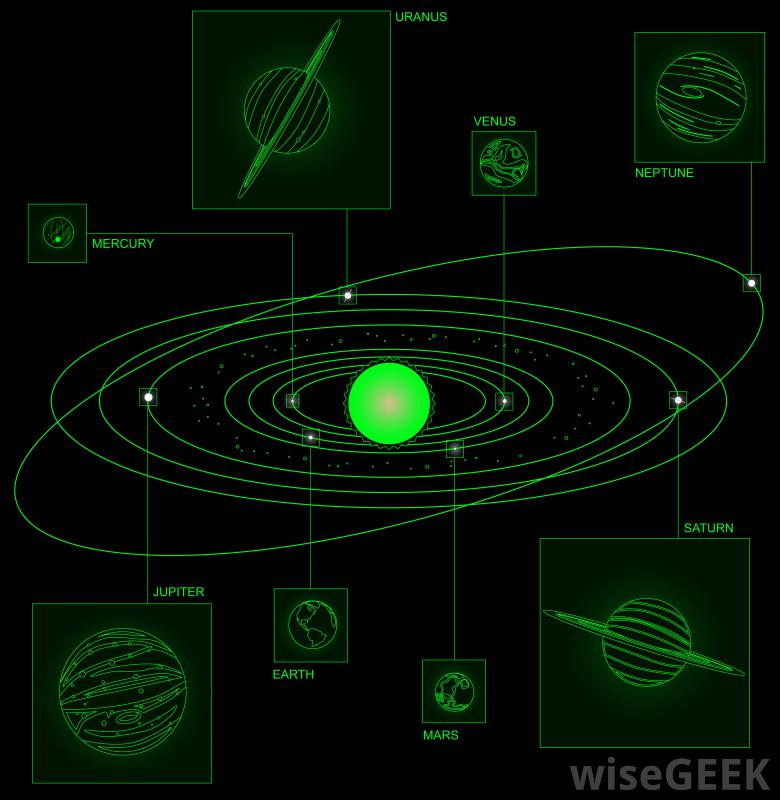
\includegraphics[scale=0.45]{Images/SolarSystem.jpg} \\[1.5cm]
		
		Florian DELRIEU \\[0.5cm]
		Diplomé en Master Dynamique des Fluides, Énergétique et Transferts \\
		Université Paul Sabatier
		
	\end{center}
\end{titlepage}

\fancyhead[L]{\leftmark}
\fancyhead[R]{\thepage}
\fancyfoot[L]{ Florian DELRIEU }
\fancyfoot[C]{}
\fancyfoot[R]{\textit{ Système Gravitationnel}}
\dominitoc
\pagenumbering{Roman}
\tableofcontents




\newpage
\pagenumbering{arabic}
%----------
\part{ Partie Théorique }
%\chapter{}
\section*{Introduction}
Ce programme a pour volonté de simuler dans un plan 2D, un système composé de $n$ corps soumis à la gravité. La programmation se fait en utilisant le code \textbf{Python} et \textbf{GitHub} (\verb!git@github.com:Florian-DELRIEU/Gravitationnal-Sytem.git!). Les différents corps seront donc en intéractions entres eux et chacun d'entre eux seront positionné de manière arbitraire avec une masse différentes.

\section*{Calcul prémiminaires}
La simulation prendra lieu dans un domaine 2D ($x$,$y$) centré sur l'origine. Dans un premier temps je vais chercher à définir le potentiel gravitationnel d'un corps dans le repère 2D. On sait que la force gravitationnelle d'un corps de masse $M$ exerce, sur un corps $m$ situé à une distance $d$, une force valant
\begin{equation}
    \vect{F_{M/m}} = - G \dfrac{M \cdot m}{d^2} \vec{u}
\end{equation}
avec $\vec{u}$ le vecteur unitaire orienté depuis le corps $M$ jusqu'au corps $m$ et $G$ étant la constante gravitationnelle.
\subsection{Ecriture du potentiel Gravitationnel}
La gravité est une force dérivant d'un potentiel que l'on va nommé $E_p$,
\begin{eqnarray}
    \vect{F_{M/m}} &=& - \Grad{E_p} \\
    \vect{F_{M/m}} &=& - \diff{E_p}{x} \vec{x} - \diff{E_p}{y} \vec{y}
\end{eqnarray}
Pour simplifier les notations je pose 
$$\vect{F_{M/m}} = \vec{F} = F_x\vec{x} + F_y\vec{y}$$
et je cherche par la suite l'expression de la composante $F_x$ uniquement car le problème est identique pour la direction $\vec{y}$
\begin{eqnarray}
    F_x &= &\diff{E_p}{x} \\
    E_p &= &\int{F_x} dx \\
    E_p &= & - G \cdot M \int{\dfrac{1}{x^2}} dx \\
    E_p &= & - G \dfrac{M}{x^3}
\end{eqnarray}
L'énergie potentielle de la force de pesanteur s'écrit alors, en faisant la similitude entre $x$ et la distance $d$ (suivant les deux composantes)
\begin{equation}
    \boxed{
    E_p =  - \dfrac{G \cdot M}{d^3}
    }
\end{equation}
\subsection{Maillage du potentiel}
Afin de visualiser ce potentiel de force dans un champs 2D, il a fallu créer un maillage rectangulaire uniforme de la forme
\begin{verbatim}
import numpy as np

dx, x_range = 0.1, 10
dy, y_range = 0.1, 10
X,Y = np.meshgrid(
    np.arange(-x_range,x_range,dx),
    np.arange(-y_range,y_range,dy))
\end{verbatim}
Une fois le maillage créé, il faut implémenter dans la programme la fonction \verb!lambda! qui représente le champs potentiel d'un objet ainsi que la position et la masse d'un objet. J'ai choisi, pour commencer
\begin{verbatim}
G = 1 # Constante Grav (6.7e8)
Pos = [(0,0)] # x,y
Mass = [1]
Potential = lambda x,y: G*Mass[0] / ( np.sqrt((x-Pos[0][0])**2+(y-Pos[0][1])**2) )**3
POTENT = Potential(X,Y)
POTENT_contour = np.linspace(POTENT.min(),POTENT.max(),10)
plt.contourf(X,Y,POTENT,[0,.1,2,5,20])
\end{verbatim}
\chapter*{Rappels de Méca}
\section*{Equation de Newton}
Les équations de la mécanique céleste sont régis par l'équation différentielle suivante
\begin{equation}
    \ddot{r} = F(r,\dot{r},t) \ann{r(t_0) = x_0 \\ \dot{r}(t_0) = v_0 }
\end{equation}
Ce système différentiel est parfaitement décris, on peut donc connaître le mouvement complet d'un corps $S$ de masse $m$. La chute libre d'un corps est décrit par la fonction
\begin{equation}
    \ddot{r} = - \mu \dfrac{r}{\norm{r}^3}
\end{equation}
avec r $\in$ $E^3$ l'ensemble des positions.
\subsection*{Trajectoire dans un champs de pesanteur central}
En écrivant le moment cinétique de $S$ au point $O$ dans son mouvement par rapport à $O$ on obtient,
\begin{equation}
    \vec H = m . \vect{OS} \wedge \vect{V_{S/R}} + \tens{I(S)}.\vect{\Omega_{S/R}}
\end{equation}
Or on ne prends pas en compte la rotation propre de $S$, on peut donc considérer que $\vect{\Omega_{S/R}} = \vec 0$, en dérivant $H$ on obtient alors
\begin{equation}
    \diff{\vec H}{t} = \diff{}{t}\left(m . \vect{OS} \wedge \vect{V_{S/R}}\right)= m \diff{\vec r}{t} \wedge \dot{\vec r} + m \vec r \wedge \diff{\dot{\vec r}}{t}
\end{equation}
$$
\diff{\vec H}{t} = m \underbrace{\dot{\vec r} \wedge {\vec r}}_{=\vec 0} + m \vec r \wedge \ddot{\vec r}
$$
\begin{equation}
    \diff{\vec H}{t} = m . \vect{OS} \wedge \vect{F} = \vec 0
\end{equation}
Le moment cinétique $\vec H$ est donc constant, le mouvement du corps $S$ est donc plan, le choix des coordonnées polaire est donc tout a fait indiqué
\chapter*{Réduction d'échelle}
\section*{Introduction}
Ce programme a pour volonté de simuler dans un plan 2D, un système composé de $n$ corps soumis à la gravité. La programmation se fait en utilisant le code \textbf{Python} et \textbf{GitHub} (\verb!git@github.com:Florian-DELRIEU/Gravitationnal-Sytem.git!). Les différents corps seront donc en intéractions entres eux et chacun d'entre eux seront positionné de manière arbitraire avec une masse différentes.

\section*{Mise à l'échelle}
\subsection*{Constante de Kepler}
Le but de cette section est de trouver un nombre adimensionnel $\mu$ afin de réduire l'échelle d'un systeme gravitationnel tout en gardant une véracité dans la simulation. Considérons le système Soleil $S$ de masse $M$, et la terre $P$ de masse $m$, orbitant à une distance $R$ (en moyenne) avec une période $T$.
\begin{equation}
    \systeme{
    M = 1.99 \times 10^{30} \text{ kg} \\
    m = 5.97 \times 10^{24} \text{ kg} \\
    R = 1.5 \times 10^{8} \text{ km} \\
    T = 3.15 \times 10^{7} \text{ s} \\
    }
\end{equation}
Avec $G$ la constante de gravitation.
Je commence par écrire l'équation du mouvement induit par la gravité soit:
\begin{equation}
    m \dfrac{d^2 r}{dt^2} = - G \dfrac{M \cdot m}{r^2}
\end{equation}
avec $G$ étant la constante gravitationnelle. $m$ se simplifiant dans l'équation, Le système est composé de 4 variables et de trois dimensions, il peut alors être réduit à un seul paramètre adimensionnel. Il existe alors une fonction $\phi$ et une variable adimensionnelle $\Pi$ telle  que
\begin{equation}
    \phi ( \Pi ) = 0
\end{equation}
Afin de le rendre adimensionnel, il n'existe qu'une combinaison de ses variables telles que 
\begin{equation}
    [M]^a [R]^b [T]^c [G]^d = 0 
\end{equation}
On obtient alors assez simplement que :
\begin{equation}
\boxed{
    \Pi = G\dfrac{M T^2}{R^3}
    }
\end{equation}
On remarque alors que nous obtenons, a une constante près, la constante de Kepler à savoir:
\begin{equation}
    \dfrac{T^2}{a^3} = \dfrac{4 \pi^2}{GM} = \text{cte}
    \label{Eq:Kepler}
\end{equation}
Ce résultat montre alors que pour tout système gravitationnel on à $\Pi = 4 \pi^2$

\subsection*{Réduction d'échelle}
Avec la connaissance de la constante de Kepler (\ref{Eq:Kepler}), il est alors facile de réduire l'échelle des grandeurs afin de simplifier les variables dans le cadre d'une simulation. Si pour simplifier je pose $G = 1 \text{ SI}$, et $a = 1 \text{ SI}$ alors on obtient la relation
\begin{equation}
\boxed{
    M = \dfrac{4 \pi^2}{T^2} 
    }
\end{equation}
Il existe alors une relation simple entre la masse du parent et la période de rotation du satellite. Si je souhaite que mon satellite ait une période de révolution autour de 2 sec (en supposant que la vitesse soit bonne) alors, la masse du parent doit être de:
$$
M = \dfrac{4 pi^2}{4} = \pi^2 = 9.86
$$
Je vais alors prendre une masse M arrondi à $10$. La période de révolution sera alors légèrement plus rapide mais toujours de l'ordre de 2 sec ($T = 1.98 \text{ s}$).
\subsection*{Vitesse orbitale}
Un satellite est en orbite circulaire autour d'un satellite si son énergie cinétique $Ec$ est égale à son énergie potentielle de pesanteur $Epp$ (a condition de le vecteur vitesse soit perpendiculaire à la direction de la force de gravité).
\begin{equation}
    Ec = Epp
\end{equation}
$$
\dfrac{1}{2} m v^2 = m g r
$$$$
v^2 = m g r
$$
avec $g = GM/r$ l'accélération de la pesanteur. On obtient alors
\begin{equation}
\boxed{
    v = \sqrt{\dfrac{2 G M}{r}}
    }
\end{equation}
Si on se place dans le cadre de notre réduction d'échelle avec $r=a$, l'expression se réduit à:
\begin{equation}
    v = \sqrt{\dfrac{2 M}{a}} = \sqrt{20}
\end{equation}
\chapter*{Mise en équation}
\section*{Formalisation}
On considère des corps $M_i$ de masse $m_i$ dans un repère en 2 dimensions $(O,\vec x,\vec y)$ repérer par le vecteur position $\vec x_i = (x_i,y_i)$, alors:
\begin{equation}
    \vect{M_i M_j} = \systeme{ x_2 - x_1 \\ y_2 - y_1}  = - \vect{M_j M_i}
\end{equation}
J'introduit le vecteur unitaire $\vec u_{ij}$ tel que:
\begin{equation}
    \vec u_{ij} = \dfrac{\vect{M_i M_j}}{\norm{\vect{M_i M_j}}}
\end{equation}
ainsi que la quantité $d_{ij} = \norm{\vect{M_i M_j}}$.

\section*{Mécanique céleste a 2 corps}
Une fois ce formalisme établie on peut alors écrire la force de gravité exercé sur un corps $i$ par un corps $j$
\begin{equation}
    \vect{F_{ij}} = G \dfrac{m_1 m_2}{\norm{\vect{M_i M_j}}^2} \vec u_{ij}
\end{equation}
\begin{equation}
    \vect{F_{ij}} = G \dfrac{m_1 m_2}{\norm{\vect{M_i M_j}}^3} \vect{M_i M_j}
\end{equation}
A ceci, je pose $\vec a_i$, $\vec v_i$ et $\vec x_i$, respectivement, l'accélération, la vitesse et la position de l'astre $M_i$ les deux corps vont alors subir les forces 
\begin{equation}
    \vect{F_{ij}} = m_i \dfrac{d^2 \vec x_i}{dt^2} = G \dfrac{m_1 m_2}{\norm{\vec x_j - \vec x_j}^3} \left( \vec x_j - \vec x_j \right)
\end{equation}

%\part{ Partie Théorique }

%\appendix
%\listoffigures
\end{document}